\documentclass[pdf,11pt]{beamer}

\usepackage[utf8]{inputenc}
\usepackage{graphicx}       % Images
\graphicspath{{Images/}}
\usepackage{xcolor}         % Change Colors
\usepackage{caption}
\captionsetup[figure]{font=small}
\usepackage{multimedia}     % Movies!
\usepackage{tikz}           % Vectored pictures
%\usepackage{media9}
%\hypersetup{pdfpagemode=FullScreen} % Presentation Mode
\usepackage{animate}        % gifs
\usepackage{tikz}
\usepackage{amsmath}
\usepackage{amssymb}
\tikzset{
    ->,
    level distance = 12em,
    minimum size=2em,
    %edge from parent/.style={draw,thick},
    level 1/.style={sibling distance=6em},
    level 2/.style={sibling distance=3em},
    thick/.style = {line width=1.5pt},
    extra thick/.style = {line width=3.5pt},
    red node/.style={shape=circle,draw=red,fill=red!40,thick,inner sep=1.2},
    blue node/.style={shape=circle,draw=blue,fill=blue!40,thick,inner sep=1.2}
}

\tikzstyle{round}=[thick,draw=black,circle]

% Remove navigation symbols
\beamertemplatenavigationsymbolsempty
% Add page number
\addtobeamertemplate{navigation symbols}{}{%
    \usebeamerfont{footline}%
    \usebeamercolor[fg]{footline}%
    \hspace{1em}%
    \insertframenumber/\inserttotalframenumber
}

% Title
\title{UO 510: Normalizing Flow Research Project
}
\author{Luis Guzman \& Steven Walton\\ \small University of Oregon}
\date{26 Mar 2020}

\usebackgroundtemplate
{
    
\includegraphics[width=\paperwidth,height=\paperheight]{UO_Simple.png}
}
\definecolor{UOYellow}{HTML}{FDCB00}
\definecolor{UOGreen}{HTML}{424443}
%\newcommand{\mytitle}[1]{\setcolor{bg=UOYellow,fg=green}\frametitle{{#1}}}

% Formatting
%\setbeamercolor{title}{fg=white}
%\setbeamercolor{normal text}{fg=white}
%\setbeamercolor{structure}{fg=white}        % Adjusts figures and frame titles
%\setbeamertemplate{frametitle}[default][center]
%\setbeamerfont{frametitle}{size=\Huge}
%%\setbeamerfont{normal text}{size=\LARGE}
%%\setbeamerfont{structure}{size=\LARGE}
%\setbeamercolor{footline}{fg=UOGreen}
%%\setbeamerfont{footline}{series=\bfseries}


\begin{document}
\frame{\titlepage}

%%%%%%%%%%%%%%%%%%%%%%%%%%%%%%
% Use include for new sections
%%%%%%%%%%%%%%%%%%%%%%%%%%%%%%

%\include{NICE}
\begin{frame}
\begin{itemize}
    \item What are Normalizing Flows
    \item NICE
    \item \textbf{\color{red}{RealNVP}}
    \item GLOW
    \item GamePlan
    \item Results
\end{itemize}
\end{frame}

\begin{frame}
    \frametitle{RealNVP (Luis)}
\end{frame}

\begin{frame}
\frametitle{GLOW}
    \begin{itemize}
        \item Flow-based generative model   
        \item Uses invertible 1x1 convolutions 
        \item Builds off of NICE and RealNVP (will leave out redundant info)
        \item Paper has a good overview of generative models and the
        differences.
    \end{itemize}
\end{frame}

\begin{frame}
\frametitle{Model}
\center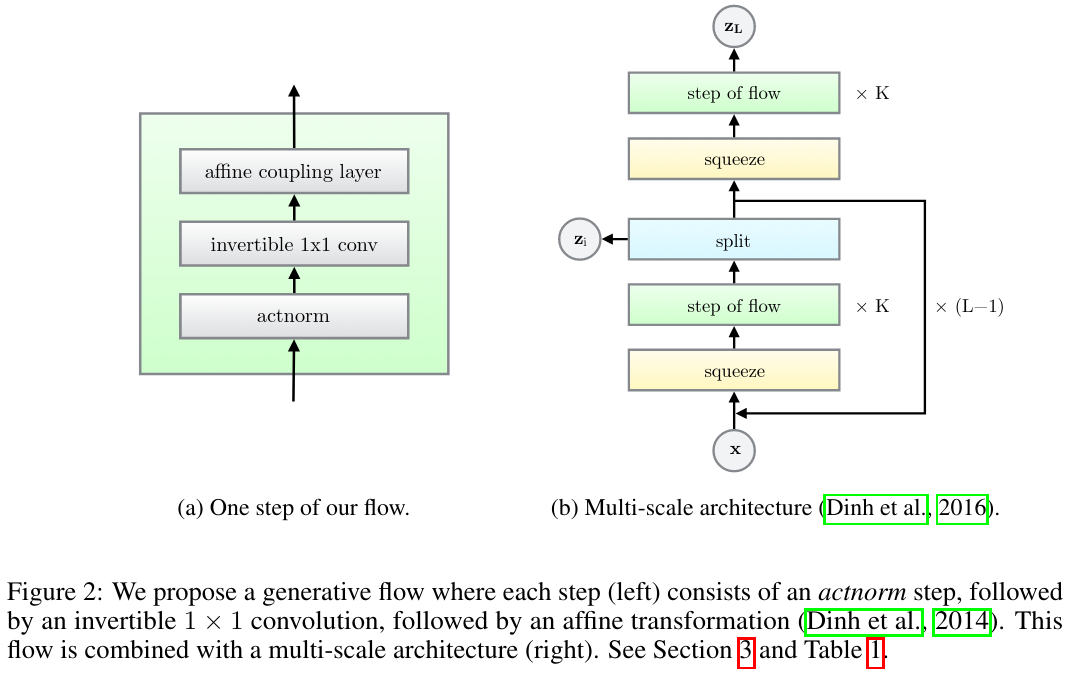
\includegraphics[width=0.8\textwidth]{GLOWModel.png}
\end{frame}

\begin{frame}
\frametitle{Model Components}
\center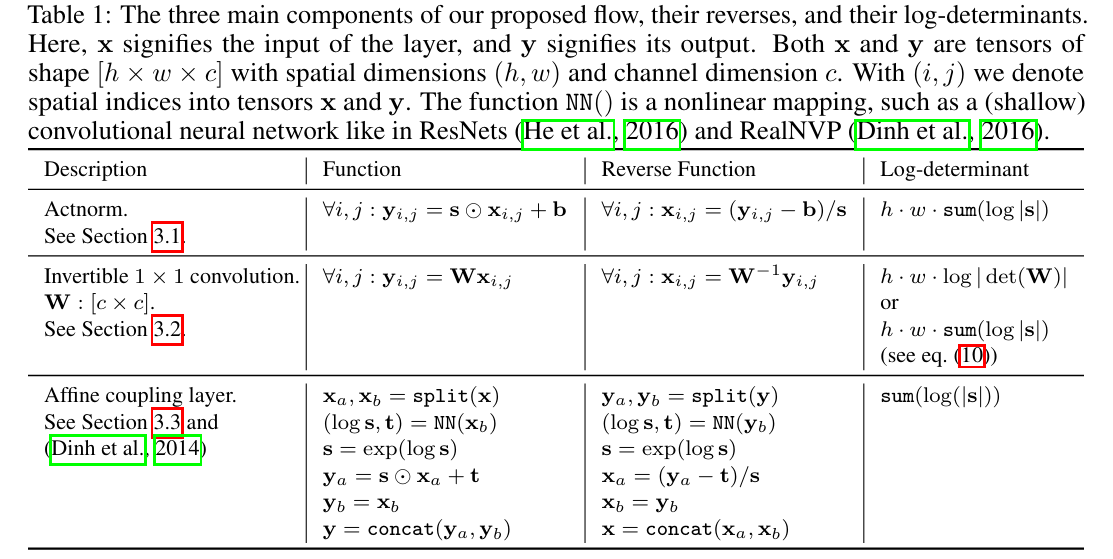
\includegraphics[width=0.8\textwidth]{GLOWComponents.png}
\end{frame}

\begin{frame}
\frametitle{Invertible 1x1 Convolutions}
    \begin{itemize}
        \item NICE uses a flow that uses a reverse permutation for channel ordering.
        \item GLOW learns this permutation with a 1x1 convolution
    \end{itemize}
    \begin{equation}
        log \left| det \left(\frac{d \textrm{conv2D}(\mathbf{h};\mathbf{W})}
                {d\mathbf{h}}\right)\right| = h \cdot w \cdot \log|det(\mathbf{W})| 
    \end{equation}
    \begin{itemize}
        \item Computing $\mathbf{W}$ can be reduced from $O(c^3)$ to $O(c)$ by
        LU Decomposition
    \end{itemize}
    \begin{align*}
        \mathbf{W} &= \mathbf{PL}(\mathbf{U} + diag(\mathbf{s}))\\
        log|det(\mathbf{W})| &= \sum(\log|\mathbf{s}|)
    \end{align*}
\end{frame}

\begin{frame}
\frametitle{Properties}
    \begin{itemize}
        \item Additive coupling layer has $\mathbf{s}=1$ and log-determinant = 0
        \item Zero initialization helps because they act like an identity
        \item Split and concatenation along channel dimension.
        \item Learned Permutation
    \end{itemize}
\end{frame}

\begin{frame}
\frametitle{GLOW Results}
\center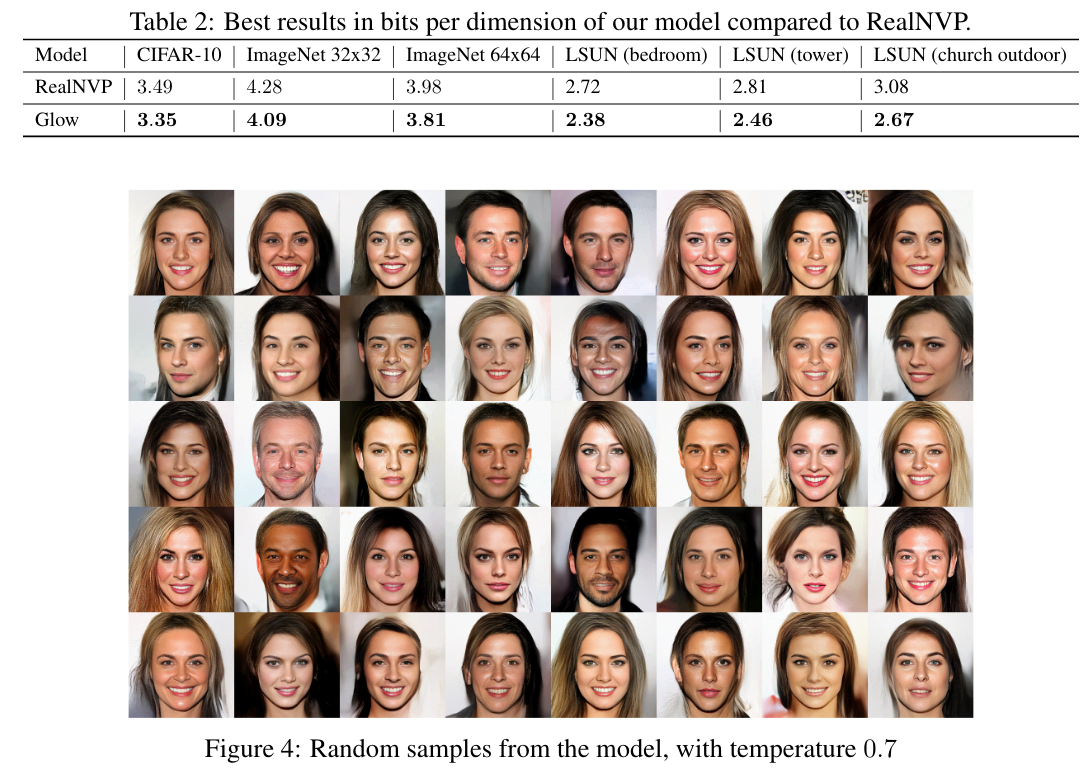
\includegraphics[width=0.8\textwidth]{GLOWResults.png}
\end{frame}

%\include{FFJORD}

\end{document}
